\documentclass[a4paper,12pt]{article}
\usepackage{amsmath,amssymb,amsfonts,amsthm}
\usepackage{tikz}
\usepackage [utf8x] {inputenc}
\usepackage [T2A] {fontenc} 
\usepackage[russian]{babel}
\usepackage{cmap} 
\usepackage{ gensymb }
% Так ссылки в PDF будут активны
\usepackage[unicode]{hyperref}
\usepackage{ textcomp }
\usepackage{indentfirst}
\usepackage[version=3]{mhchem}

% вы сможете вставлять картинки командой \includegraphics[width=0.7\textwidth]{ИМЯ ФАЙЛА}
% получается подключать, как минимум, файлы .pdf, .jpg, .png.
\usepackage{graphicx}
% Если вы хотите явно указать поля:
\usepackage[margin=1in]{geometry}
% Или если вы хотите задать поля менее явно (чем больше DIV, тем больше места под текст):
% \usepackage[DIV=10]{typearea}

\usepackage{fancyhdr}

\newcommand{\bbR}{\mathbb R}%теперь вместо длинной команды \mathbb R (множество вещественных чисел) можно писать короткую запись \bbR. Вместо \bbR вы можете вписать любую строчку букв, которая начинается с '\'.
\newcommand{\eps}{\varepsilon}
\newcommand{\bbN}{\mathbb N}
\newcommand{\dif}{\mathrm{d}}

\newtheorem{Def}{Определение}


\pagestyle{fancy}
\makeatletter % сделать "@" "буквой", а не "спецсимволом" - можно использовать "служебные" команды, содержащие @ в названии
\fancyhead[L]{\footnotesize Оптика}%Это будет написано вверху страницы слева
\fancyhead[R]{\footnotesize ФМХФ МФТИ}
\fancyfoot[L]{\footnotesize \@author}%имя автора будет написано внизу страницы слева
\fancyfoot[R]{\thepage}%номер страницы —- внизу справа
\fancyfoot[C]{}%по центру внизу страницы пусто

\renewcommand{\maketitle}{%
	\noindent{\bfseries\scshape\large\@title\ \mdseries\upshape}\par
	\noindent {\large\itshape\@author}
	\vskip 2ex}
\makeatother
\def\dd#1#2{\frac{\partial#1}{\partial#2}}


\title{4.2.3 \\ Интерферометр Релея}
\author{Егор Берсенев} 
\date{16 февраля 2017 г.}

\begin{document}
	
	\maketitle
	\section{Цель работы}
	Ознакомление с устройством и принципом действия интерферометра Релея и с его применением для измерения показателей преломления газов.
	\section{Оборудование}
	Технический интерферометр ИТР-1, светофильтр, баллон с углекислым газом, сильфон, манометр, краны.
	\section{Теоретическая часть}
	В интерферометре Релея используется дифракция Фраунгофера на двух щелях. Используя принцип Гюйгенса-Френеля рассчитаем интенсивность световых колебаний в волне, направление распространения которой составляет угол $\varphi$ с нормалью к экрану. Элемент щели $\dif x$ посылает в направлении $\varphi$ волну с амплитудой, пропорциональной $\dif x$. Фаза волны, приходящей в точку наблюдения от элемента с координатой $x$, отстает от фазы волны, приходящей с $x = 0$, на величину $kx\sin\varphi$. Колебание $\dif E$ в точка наблюдения, вызванное элементом $\dif x$, может быть записано в виде:
	\begin{equation}
	\dif E = a\cos\left(\omega t - kx\sin\varphi\right)\dif x
	\end{equation}
	
	Найдем результат $E$ суммарного действия всех элементов обоих щелей. Будем при этом считать, что в правой щели создана дополнительная разность хода $\Delta$, одинаковая для всех ее элементов. Интегрируя, получим:
	\begin{equation}
	E = \int_{0}^{b} a\cos\left(\omega t - kx\varphi\right)\dif x + \int_{d}^{d + b} a\cos\left(\omega t - kx\varphi - k\Delta\right)\dif x
	\end{equation}
	Получаем:
	\begin{equation}
	E =2ab \cfrac{\sin\left(\cfrac{kb\varphi}{2}\right)}{\cfrac{kb\varphi}{2}}\cos\frac{k\Delta + kd\varphi}{2}\cos\left(\omega t - \frac{k\Delta + k\left(d+b\right)\varphi}{2}\right)
	\end{equation}
	Отсюда интенсивность:
	\begin{equation}
	I = 2I_0\left[\cfrac{\sin\left(\cfrac{kb\varphi}{2}\right)}{\cfrac{kb\varphi}{2}}\right]^2\left(1+\cos\left(k\Delta + kd\varphi\right)\right)
	\end{equation}
	Интерференционные максимумы отстоят друг от друга на равные угловые расстояния:
	\begin{equation}
	\delta\varphi = \frac{\lambda}{d}
	\end{equation}
	
	\subsection{Описание установки}
	Схема прибора представлена на рисунке 1 в вертикальной и горизонтальной проекциях. Лампа накаливания Л с помощью конденсора К ярко освещает узкую входную щель S, расположенную в фокусе объектива $O_1$. Коллиматор, состоящий из щели $S$ и объектива $O_1$, посылает параллельный пучок на диафрагму $D$ с двумя вертикальными щелями. Свет, дифрагируя на двойной щели проходит кювету $L$, состоящую из двух одинаковых стеклянных камер, в которые вводятся исследуемые газы. Кювета занимает только верхнюю часть пространства между объективами. За кюветой расположены две стеклянных пластинки $J$ и пластинка П. 
	
	Дифракционная картина, образующая в фокальной плоскости $F$ объектива $O_2$, рассматривается через окуляр $O$.
	
	\begin{figure}[h!]
		\begin{center}
			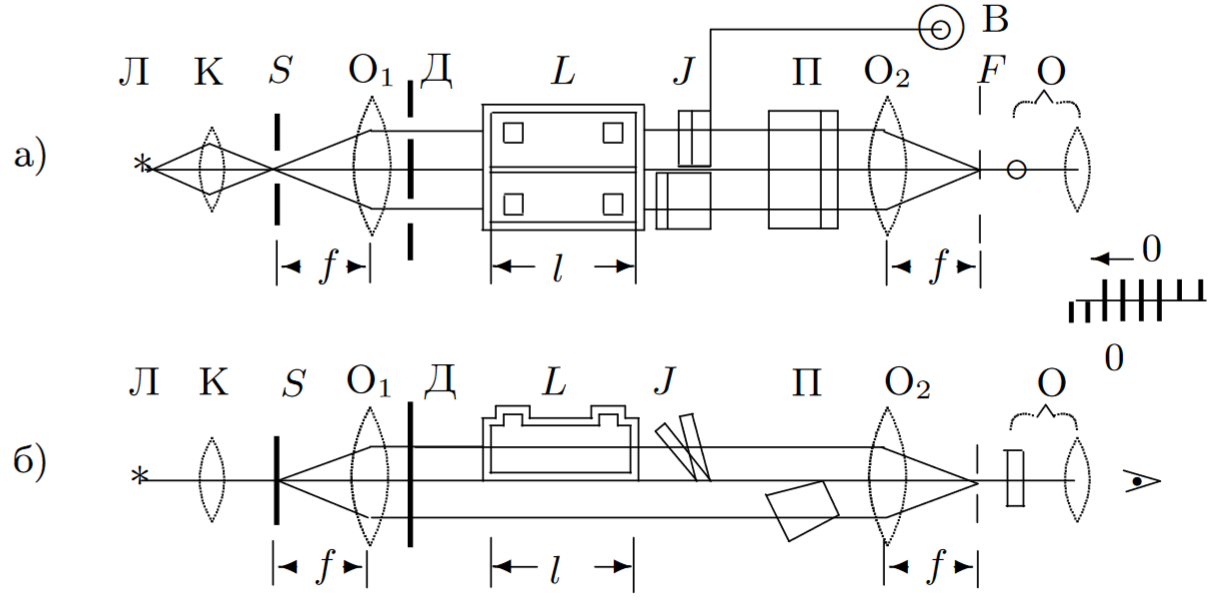
\includegraphics[width = \linewidth]{expsc}
			\caption{Схема установки: а) вид сверху, б) вид сбоку}
		\end{center}
	\end{figure}
	
	При заполнение камер газами с одинаковым показателем преломления $n$ системы полос совпадают. Разность хода $\Delta = \Delta n \cdot l$, возникает при прохождении света через камеры с разными газами и ведет к смещению полос. Смещение на одну полосу соответствует дополнительной разности хода $\Delta = \lambda$. Просчитав число полос между центрами можно рассчитать:
	\begin{equation}
	\Delta n = \frac{\Delta}{l} = m\frac{\lambda}{l}
	\end{equation}
	
	\subsection{Зависимость показателя преломления газа от давления и температуры}
	Известно простое соотношение между показателем преломления газа и его плотностью:
	\begin{equation}
	n = \sqrt{\varepsilon} = \sqrt{1+4\pi N\alpha} \simeq 1 + 2\pi N \alpha
	\end{equation}
	Принимая во внимание $p = NkT$, получаем:
	\begin{equation}
	n - 1 = 2\pi\alpha\frac{P}{kT}
	\end{equation}
	Отсюда следует, что при постоянной температуре изменение показателя преломления $\Delta n$ пропорционально изменению давления $\Delta P$.
	\begin{equation}
	\Delta n = \frac{2\pi\alpha}{kT}\Delta P
	\end{equation}
	
	\section{Экспериментальная часть}
	Длина кюветы $l = 10 \,\text{см}$, атмосферное давление $P = 101.2\cdot 10^3\,\text{Па}$, температура $T = 21 \degree C$. Прокалибруем установку в единицах $\lambda$. Для этого построим график смещения от номера полосы:
	
	\begin{figure}[h!]
		\begin{center}
			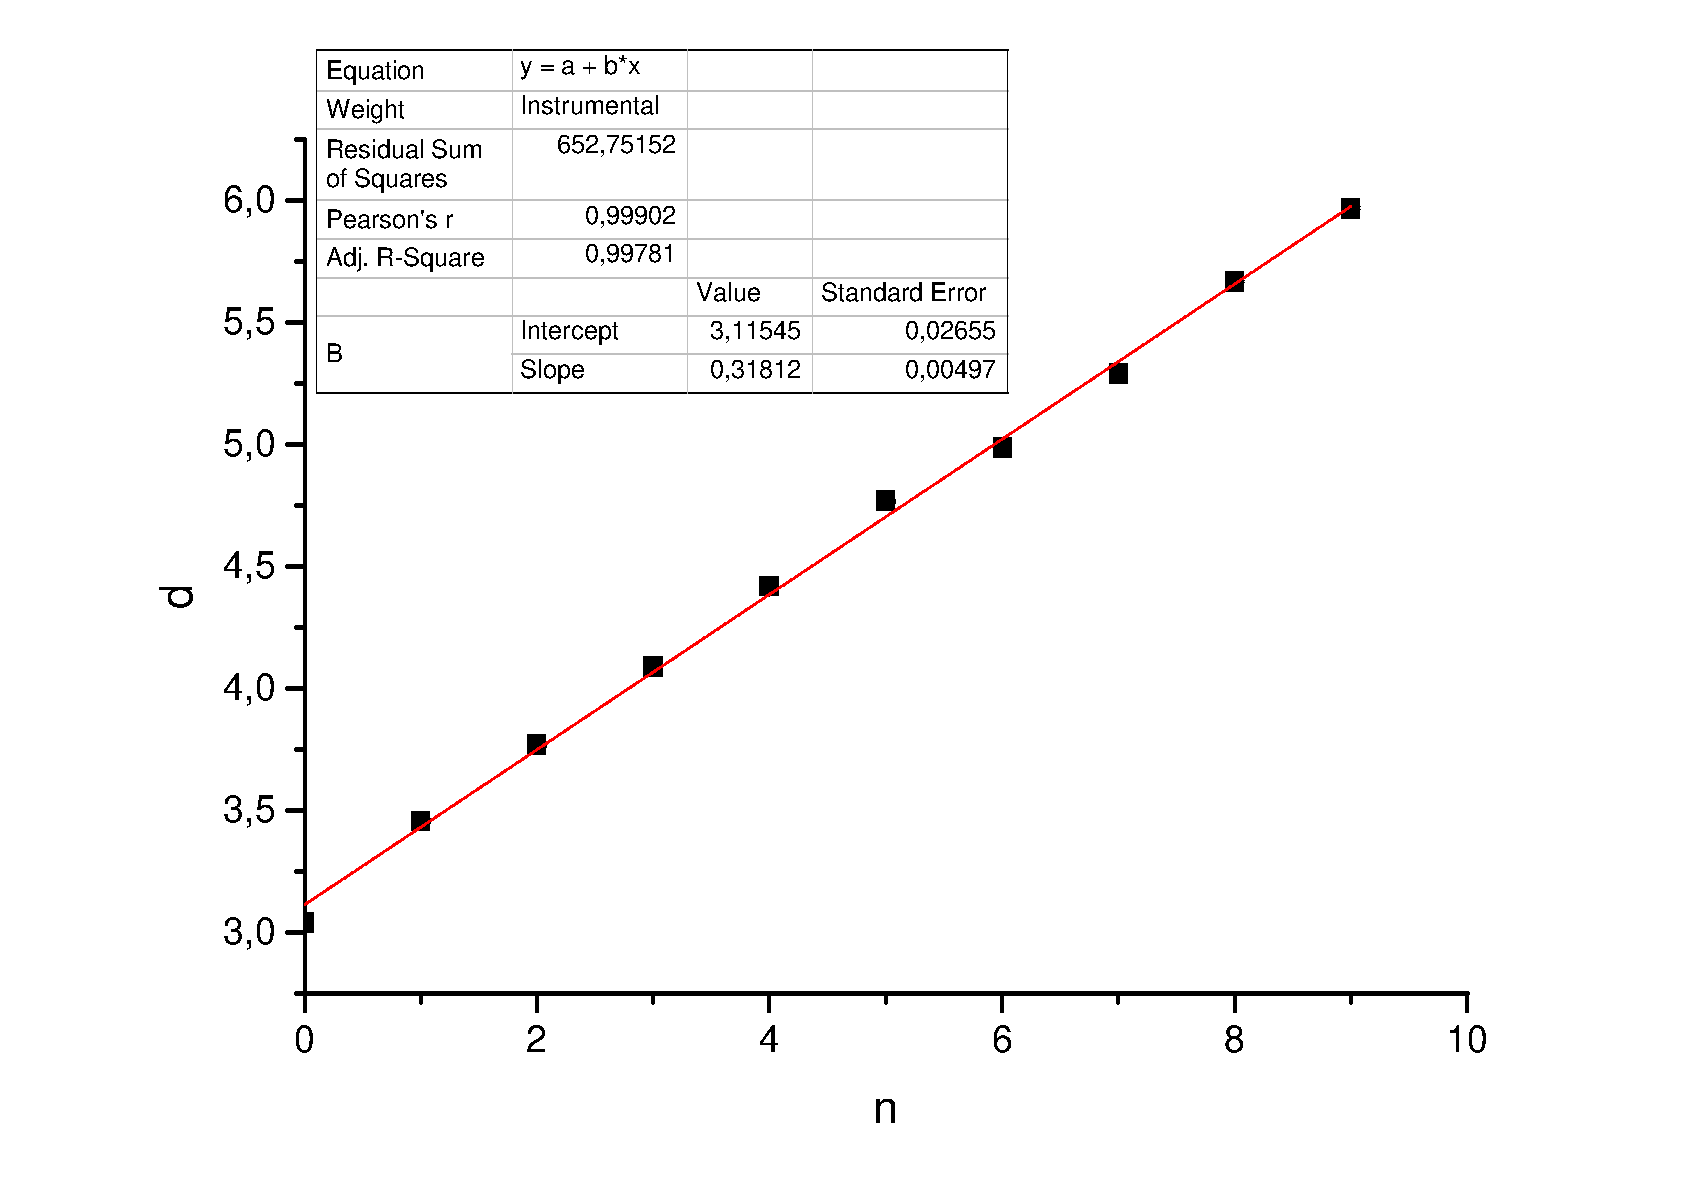
\includegraphics[width = \linewidth]{dn}
			\caption{Зависимость смещения от номера полосы}
		\end{center}
	\end{figure}
	\newpage
	Будем использовать калибровочный график для расчета $\Delta n$. Таким образом построим график в координатах $\Delta n\left(\Delta P\right)$.
	
	\begin{figure}[h!]
		\begin{center}
			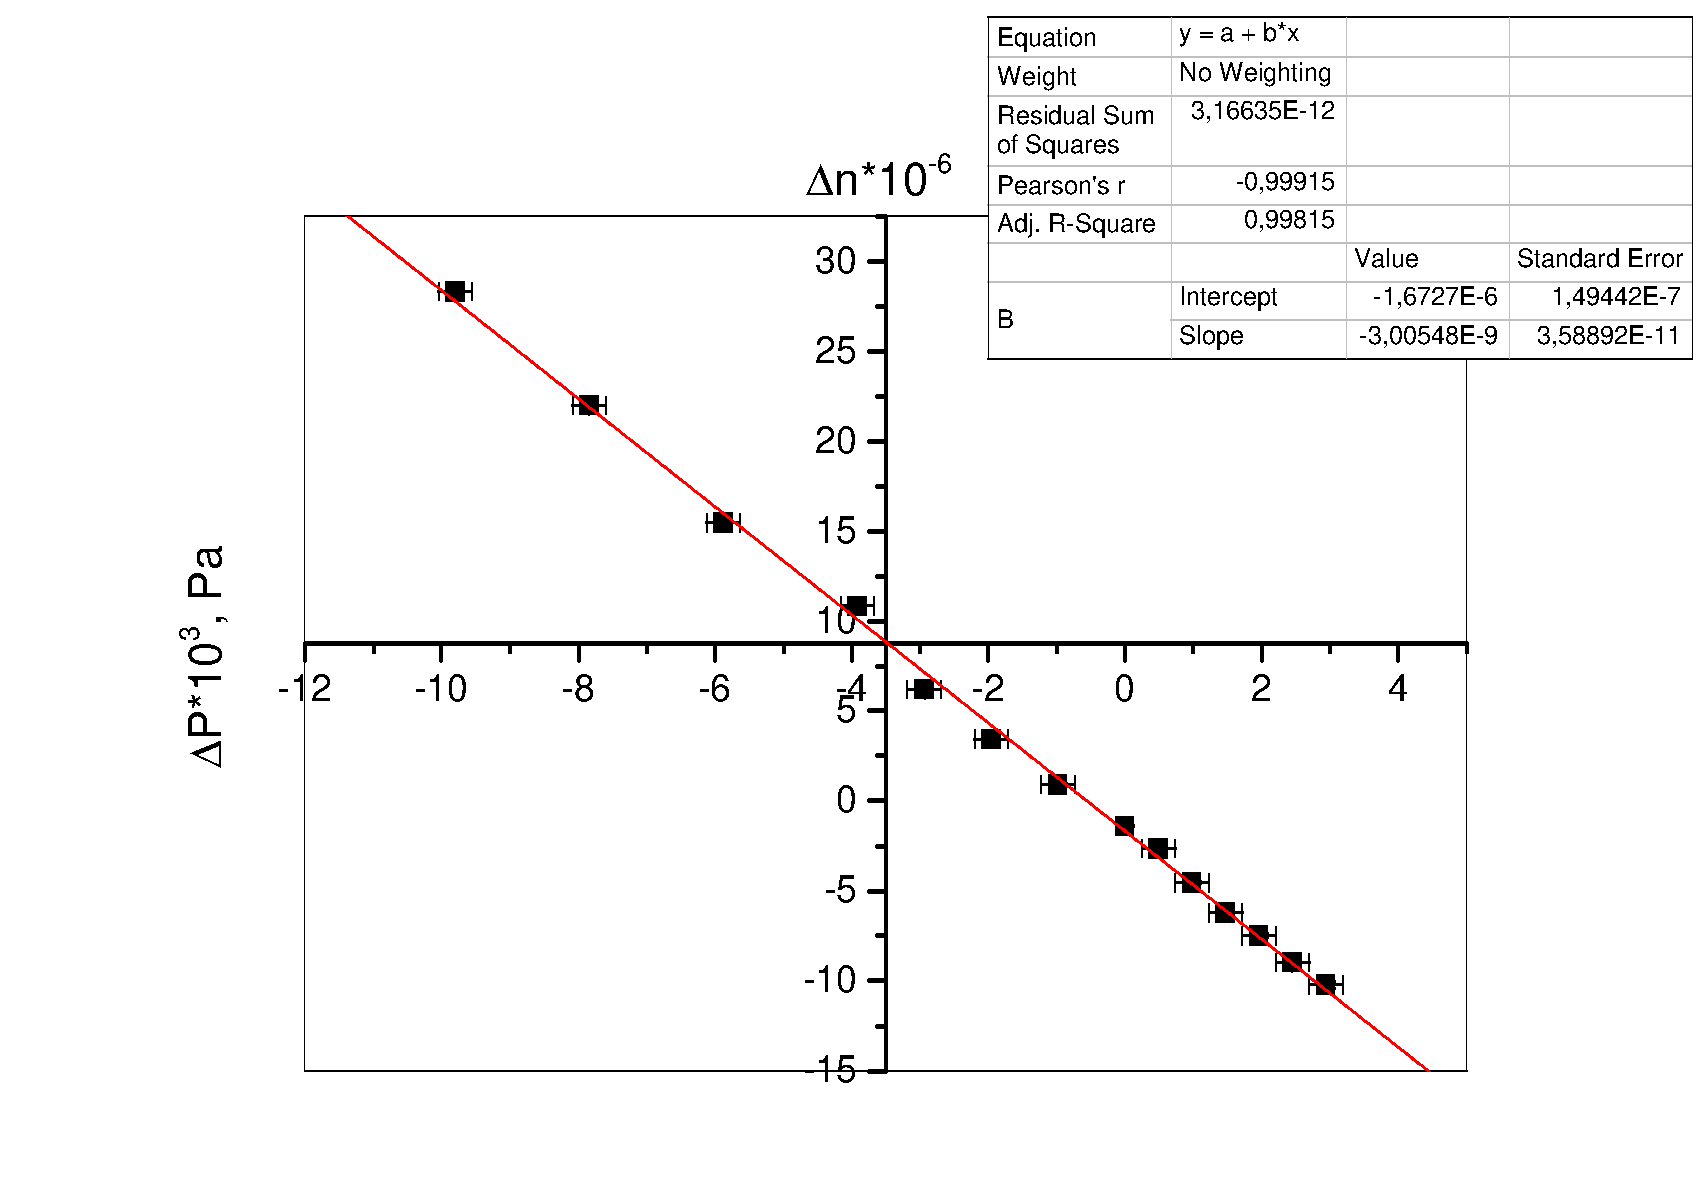
\includegraphics[width = \linewidth]{dndp}
			\caption{Зависимость показателя преломления от перепада давлений}
		\end{center}
	\end{figure}
	
	Отсюда получаем показатель преломления воздуха. пересчитанный к нормальным условиям $ n_0 = 1.0003\pm 0.00005$, что сходится с табличным результатом в пределах погрешности($n_{0_{t}} = 1.0002929$)
	
	Теперь заполним кювету углекислым газом, и пронаблюдаем зависимость смещения компенсатора от времени:
	
	\begin{figure}[h!]
		\begin{center}
			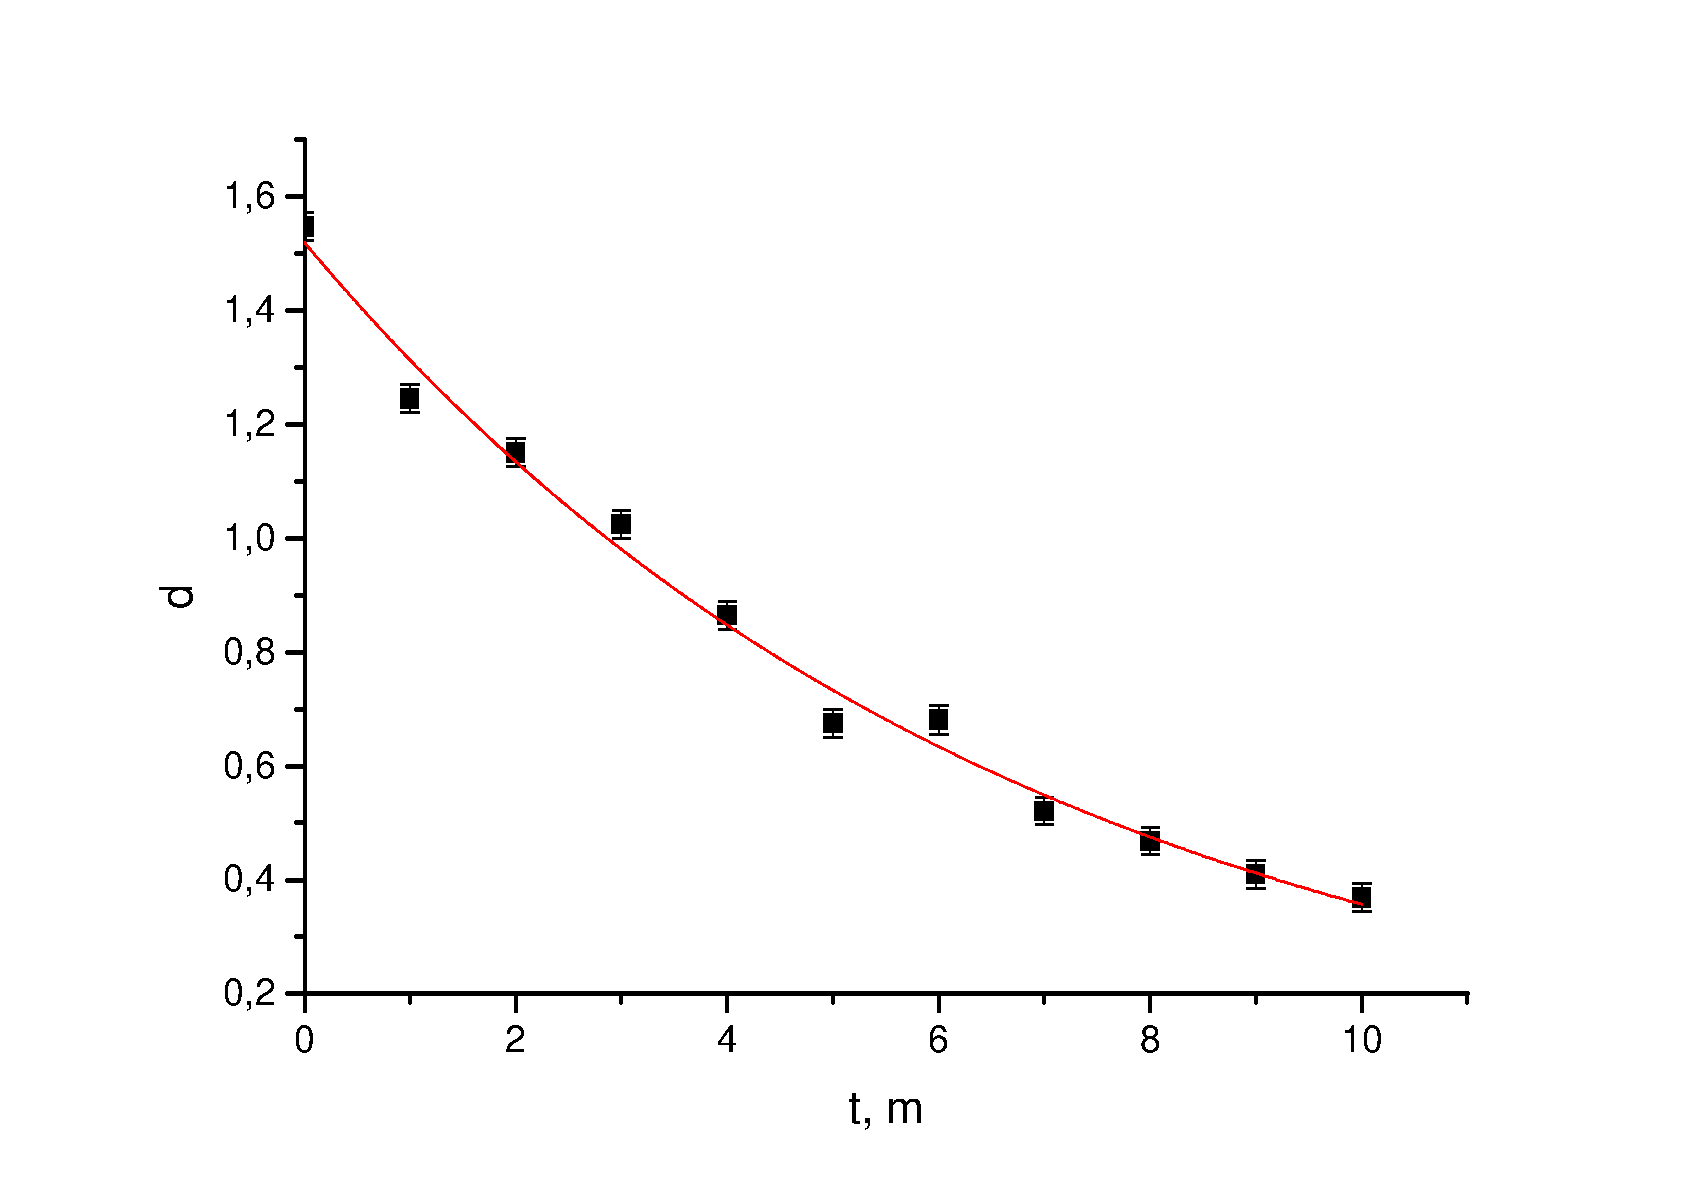
\includegraphics[width = \linewidth]{dt}
			\caption{Зависимость смещения компенсатора от времени}
		\end{center}
	\end{figure}
	
	Равновесие устанавливается очень долго, следовательно концентрация \ce{CO2} в каждый момент времени не очень понятна. Поэтому будем заполнять кювету углекислым газом медленно, во избежание изменения температуры при расширении газа и рассчитаем показатель преломления по одной начальной точке:
	
	
	\begin{table}[h!]
		\centering
		\caption{Расчет показателя преломления}
		\label{my-label}
		\begin{tabular}{|l|l|l|l|}
			\hline
			& d     & $\Delta n$ & n          \\ \hline
			1 & 10.55 & 0.000157   & 1.000457 \\ \hline
			2 & 10.46 & 0.000155   & 1.000455 \\ \hline
			3 & 10.48 & 0.000155   & 1.000455 \\ \hline
			4 & 10.46 & 0.000155   & 1.000455 \\ \hline
			5 & 10.53 & 0.000156   & 1.000456 \\ \hline
		\end{tabular}
	\end{table}
	
	\newpage
	
	
	Итого $n = 1.00045 \pm 0.00002$. Табличный показатель преломления для \ce{CO2} $n_0 = 1.00045$, что также сходится с нашими измерениями.
	
	\section{Вывод}
	Интерферометр Релея позволяет измерять разность показателей преломления в двух кюветах с высокой точностью. Для таких измерений нужно поддерживать давление в кюветах и концентрацию газа постоянной, в противном случае точность и простота измерений значительно ухудшаются.
	

	

\end{document}


